\documentclass{article}

\title{Graphics P2}
\date{23/04/2019}
\author{150008859}

\setlength{\parskip}{1em}
\setlength{\parindent}{0em}

\usepackage{listings}
\usepackage{amsmath,amssymb,amsthm}
\usepackage{mathtools}
\usepackage{graphicx}
\usepackage{subfigure}
\usepackage{xcolor}


\begin{document}
\maketitle

\section{Introduction}

For this practical, I implemented the following elements.

\begin{enumerate}
\item Rendering and Interpolating of 3 Faces.
\item Flat Shading and Lighting using Lambert's Reflectance model.
\item Perspective Projection.
\end{enumerate}

Furthermore, the extensions include the following.

\begin{enumerate}
\item Backface Culling
\item Face rotation
\item Swapping of Faces
\end{enumerate}

No external libraries are used. 

The tools are written in Java using the matrix and camera library developed in the previous practical.

Place ``CS4102 2019 P2 data'' in the Graphics2 folder. 

Run the 3d tool by running the following command. 

\begin{verbatim}
java -cp bin graphics.draw.Draw
\end{verbatim}

Control the fps camera  by using ``wsda'' and the ``arrow keys'' (the origin of light is the camera's position).

Rotate the face around the y axis by using ``jk'' (the lighting does not account for rotation).

Swap a face by hitting 1, 2 or 3 on the keyboard to select a face and enter a face number from 1 to 199.

Alter the weights by \textbf{dragging} the circle in triangle.

\begin{figure}%
\centering
\subfigure[Example 1]{%
  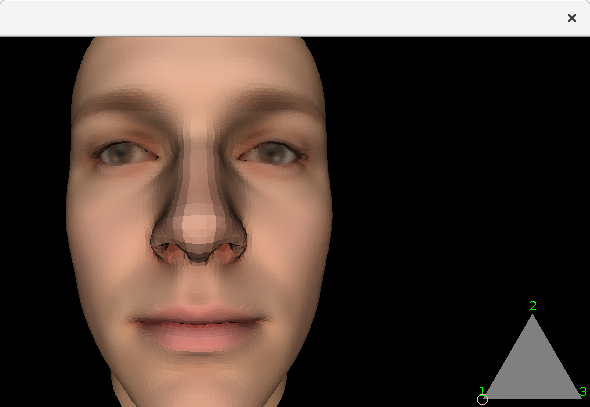
\includegraphics[scale=0.2]{images/image1.png}}%
\qquad
\subfigure[Example 2]{%
  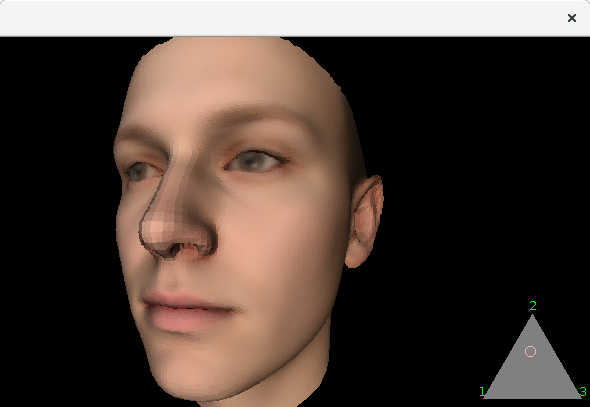
\includegraphics[scale=0.2]{images/image2.png}}%
\qquad
\subfigure[Example 3]{%
  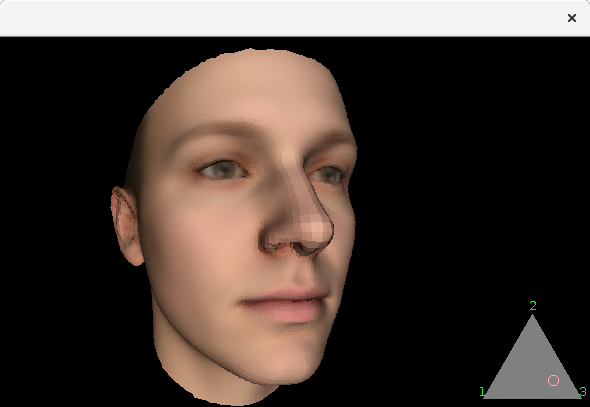
\includegraphics[scale=0.2]{images/image3.png}}%
\caption{A demonstration of the application.}
\end{figure}

\begin{figure}[ht!]
\centering
\subfigure[Example 1]{%
  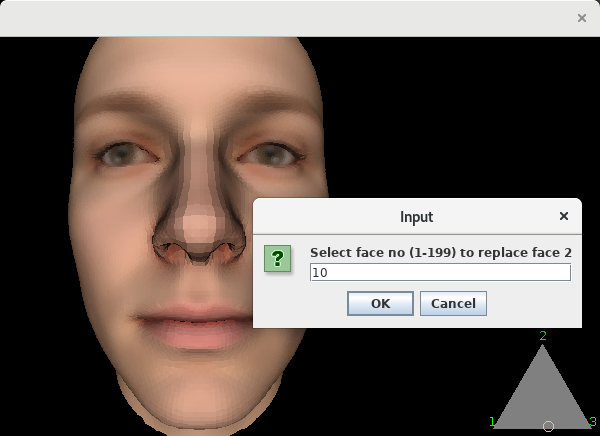
\includegraphics[scale=0.2]{images/replace1.png}}%
\qquad
\subfigure[Example 2]{%
  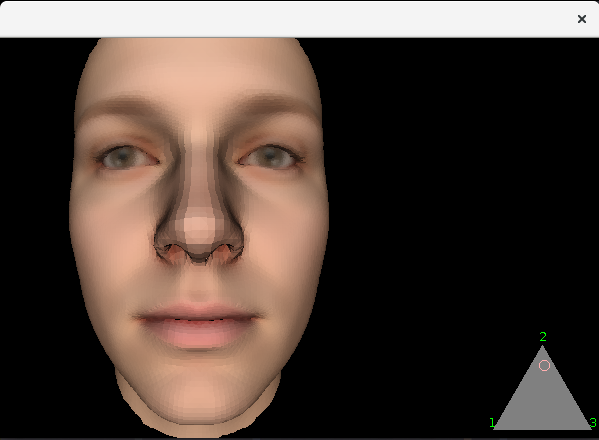
\includegraphics[scale=0.2]{images/replace2.png}}%
\caption{Swapping faces.}
\end{figure}

\section{The basic specification}

\subsection{Rendering}

The vertex and colour data supplied is loaded, scaled to fit between approximately $(-1, 1)$ and assembled into triangles consisting of 3 vertices (each vertex using the homogeneous coordinate system) and 3 texture elements. A face consists of a collection of these triangles.

A model matrix is constructed for the purposes of scaling, rotation and translation. A view matrix is constructed using the camera's position, target and the ``up'' axis which is y. A right handed coordinate system is used with the camera looking down towards the negative z axis. Next, a perspective projection matrix is configured with the height and width to calculate the aspect ratio, an angle to specify the field of view and the near and far clipping planes.

A new matrix is assembled by performing the multiplication $ m = \mathit{projection} * \mathit{view} * \mathit{model} $. The vertices of the triangle are multiplied by this matrix $ t_i = m v_i $, resulting in the vertices of the triangle going from local space to clip space.

I adapted some elements of my matrix library to minimise memory allocations. I tried several implementations for this practical in which I experimented with using simple arrays of native types to store vertices, however, I settled with a more object oriented approach as the performance difference was minimal and the code was more readable. 

In the next step called the perspective divide, the x, y and z elements are divided the w element of the vector. A copy of z (the depth) is saved in the slot occupied by w. This is equivalent to giving smaller vertex coordinates to a vertex that is further away from the viewier. Finally, a small calculation is performed to go from clip space to screen space.

Next the triangles are sorted using the value of z (the depth) that we stored in the w slot, this is called the painter's algorithm in which triangles further away from the viewer are drawn first with closer triangles being drawn over. The sorting is performed by using Java's ``Collections.sort''.



\subsection{Shading}

A flat shading model along with Lambert's reflectance model is used to select the colour of a triangle.

The colour of each triangle is the average of the supplied colour values. 

A surface normal is calculated by taking the cross product of two lines in the triangle.

The direction of incident light is the average position of the triangle subtracted by the camera's position.

A diffuse value is calculated by taking the dot product of the surface normal and the direction of light.

The RGB components of each triangle are scaled by the diffuse value to produce the final colour value of the triangle.

\subsection{Interpolation of Faces and the Triangle}

The weights are calculated using the barycentric coordinate system as the basis of the calculation \cite{interpolation}. I am unfamiliar with how this technique works, but it was superior to the more naive distance technique that I was originally going to use as it works for all cases. A flaw of the naive system is exposed when using a non equilateral triangle. 

The vertices and the texture elements of the new average face are calculated by taking the weighted average of the vertices and textures of the faces that it consists of. New surface normals and light directions are calculated for each of the new triangles in the new face. 

\section{Extensions}

\subsection{Backface Culling}

The orientation of the triangle is determined by calculating the determinant of a 2x2 matrix containing $p_2 - p_1$ and $p_3 - p_2$ \cite{orientation}. This returns a positive or negative value if the vertices of the triangle are clockwise (a forward facing triangle) or counter clockwise (a backwards facing triangle). Backwards facing triangles are not drawn.

The triangle is front facing if the following calculation is less than zero.

$\ (y_2 - y_1) * (x_3 - x_2) - (x_2 - x_1) * (y_3 - y_2) $

\subsection{Rotation of the Face}

The user can rotate the face by using the ``jk'' keys, one small flaw is that the direction of the light is not accounted for when rotating so it appears as if the light source is moving when the face is rotated. This is because I am performing the light calculation on the data before it is rotated. Rotation is performed by multiplying the coordinates of the face by a rotation matrix before the view and projection matrices are applied. 

\subsection{Swapping of Faces}

Suppose you are swapping face 3 with a new face, face 1 and face 2 are averaged with the current average face and the new face replaces face 3. This stores the accumulation of the current faces and allows the new face to contribute to the currently accumulated face. A small flaw with this is that faces 1 and 2 will become similar over time. I cannot currently think of a better technique is the current accumulation of the face needs to be shared with the other two faces. 

\begin{thebibliography}{5}
  
\bibitem{interpolation}
  Triangular Interpolation using the barycentric coordinates system
  \\\texttt{https://codeplea.com/triangular-interpolation}

\bibitem{coordinate}
  Barycentric coordinate system
  \\\texttt{https://en.wikipedia.org/wiki/Barycentric\_coordinate\_system}

\bibitem{orientation}
  Orientation of polygon
  \\\texttt{https://cp-algorithms.com/geometry/oriented-triangle-area.html}

  
\end{thebibliography}




\end{document}
